\documentclass[11pt]{article}
    %	options include 12pt or 11pt or 10pt
    %	classes include article, report, book, letter, thesis

    \usepackage{amsmath}
    \usepackage{array}
    \setlength\extrarowheight{2pt}
    \usepackage{graphicx}
    \usepackage{epstopdf}
    \usepackage{graphics}
    \graphicspath{ {/home/shanedrafahl/coms331/hw0} }
    
    \title{HW3}
    \author{Shane Drafahl}
    \date{20 October,2017}

    \begin{document}
    \maketitle

    1. (a) 
    $ \newline $

    \begin{figure}[!htb]
        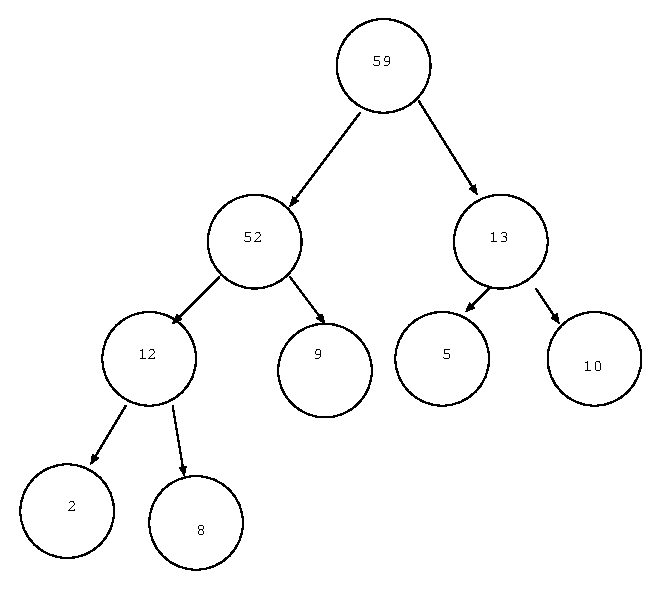
\includegraphics[scale=.7]{./maxheap.eps}
    \end{figure}

    $ \newline $

    First we will replace the removed element with the last element in the tree

    (b): 

    $ \newline $

    \begin{figure}[!htb]
        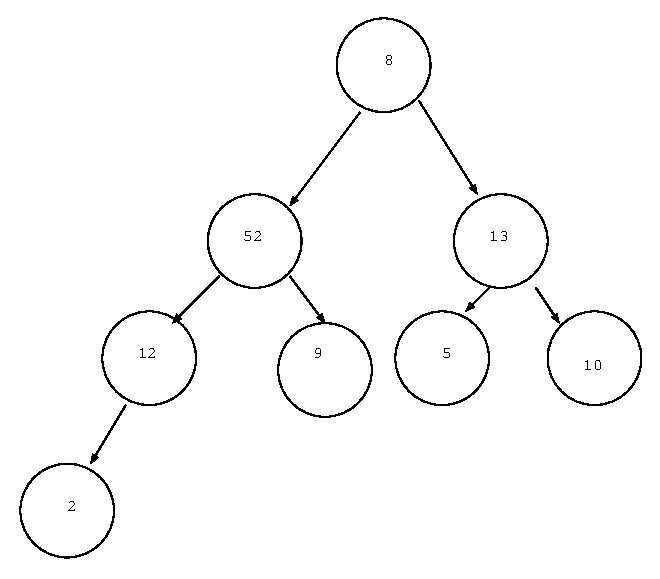
\includegraphics[scale=.7]{./removeHeap.eps}
    \end{figure}

    $ \newline $

    Then we must heapify the data structure

    \begin{figure}[!htb]
        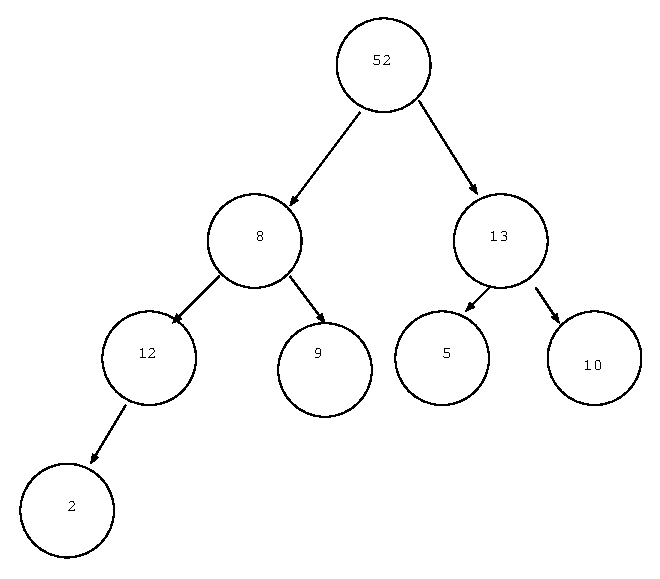
\includegraphics[scale=.7]{./removeMax2.eps}
    \end{figure}

    $ \newline $

    \begin{figure}[!htb]
        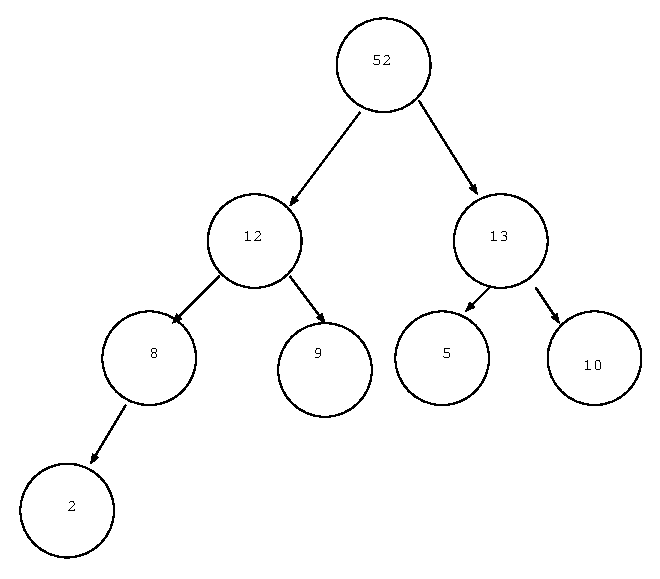
\includegraphics[scale=.7]{./removeMax3.eps}
    \end{figure}

    $ \newline $

    The max heap is now been heapified.

    $ \newline $

    2. Solve the following recurrences. You can not use master theorem to solve them. You must
    show the steps in your derivation.

    $ \newline $

    (a):  If we draw out a 3 iterations then we would get
    $ \newline $
    $ [cn]_{1} + [\frac{cn}{3} + \frac{2cn}{3}]_{2}]_{2} + [\frac{cn}{9} + \frac{2cn}{9} + \frac{2cn}{9} + \frac{4cn}{9}]_{3} $
    $ \newline $
    where the brackets represent the layers this can be reduced to $ [cn]_{1} + [cn]_{2} + [cn]_{3} + ... $ for all iterations.
    So now we just need to find the number of iterations. Every iteration divides n by 3 or by $ \frac{2}{3} $. So there should
    be logarithmic number of iterations. So $ T(n) = cnlog(n) $.
    $ \newline $
    

    

    \end{document}
